\documentclass[11pt,english,compress]{beamer}

\usepackage[utf8]{inputenc}
\usepackage{verbatim}
\usepackage{eurosym}
\usepackage{stmaryrd}

\usepackage[compatibility=false]{caption}
\usepackage{subcaption}
\usepackage{pgfplots}

\useoutertheme[subsection=false]{smoothbars}
\useinnertheme[shadow=true]{rounded}

\usecolortheme{orchid}
\usecolortheme{whale}

\setcounter{tocdepth}{2}
\setcounter{secnumdepth}{0}

\setbeamertemplate{footline}[frame number]

\title{The Linux graphics stack, Optimus and the Nouveau driver}
\subtitle{Cooperative rendering across GPUs on Linux}
\author{Martin Peres}
\institute{Nouveau developer\\PhD student at LaBRI\\X.Org Foundation board member}

\AtBeginSection[]{
  \begin{frame}{Summary}
  \small \tableofcontents[currentsection, hideothersubsections]
  \end{frame} 
}

\begin{document}

\setbeamertemplate{navigation symbols}{}
\setbeamertemplate{footline}[frame number]

\begin{frame}[plain,noframenumbering]
	\titlepage
\end{frame}

\section{Introduction to the Linux graphics stack}
\subsection{General overview}
\begin{frame}
	\frametitle{General overview of the Linux Graphics stack}

	\begin{block}{The graphics stack before 2005}
		\begin{itemize}
			\item The X-Server provided everything:
			\begin{itemize}
				\item Modesetting (CRTC \& plane management);
				\item 2D/3D acceleration;
				\item Video rendering acceleration;
				\item Input management.
			\end{itemize}
			\item The X-Server talked to the GPU directly, as root.
		\end{itemize}
	\end{block}

	\begin{block}{The current graphics stack}
		\begin{itemize}
			\item The X-Server got split into more than 200 components:
			\begin{itemize}
				\item Privileged operations moved to the kernel;
				\item 2D drivers got put into different shared objects;
				\item 3D acceleration got put in mesa;
				\item The list is too long (and boring) ;)
			\end{itemize}
		\end{itemize}
	\end{block}
\end{frame}

\begin{frame}
	\begin{figure}[h]
		\centering
		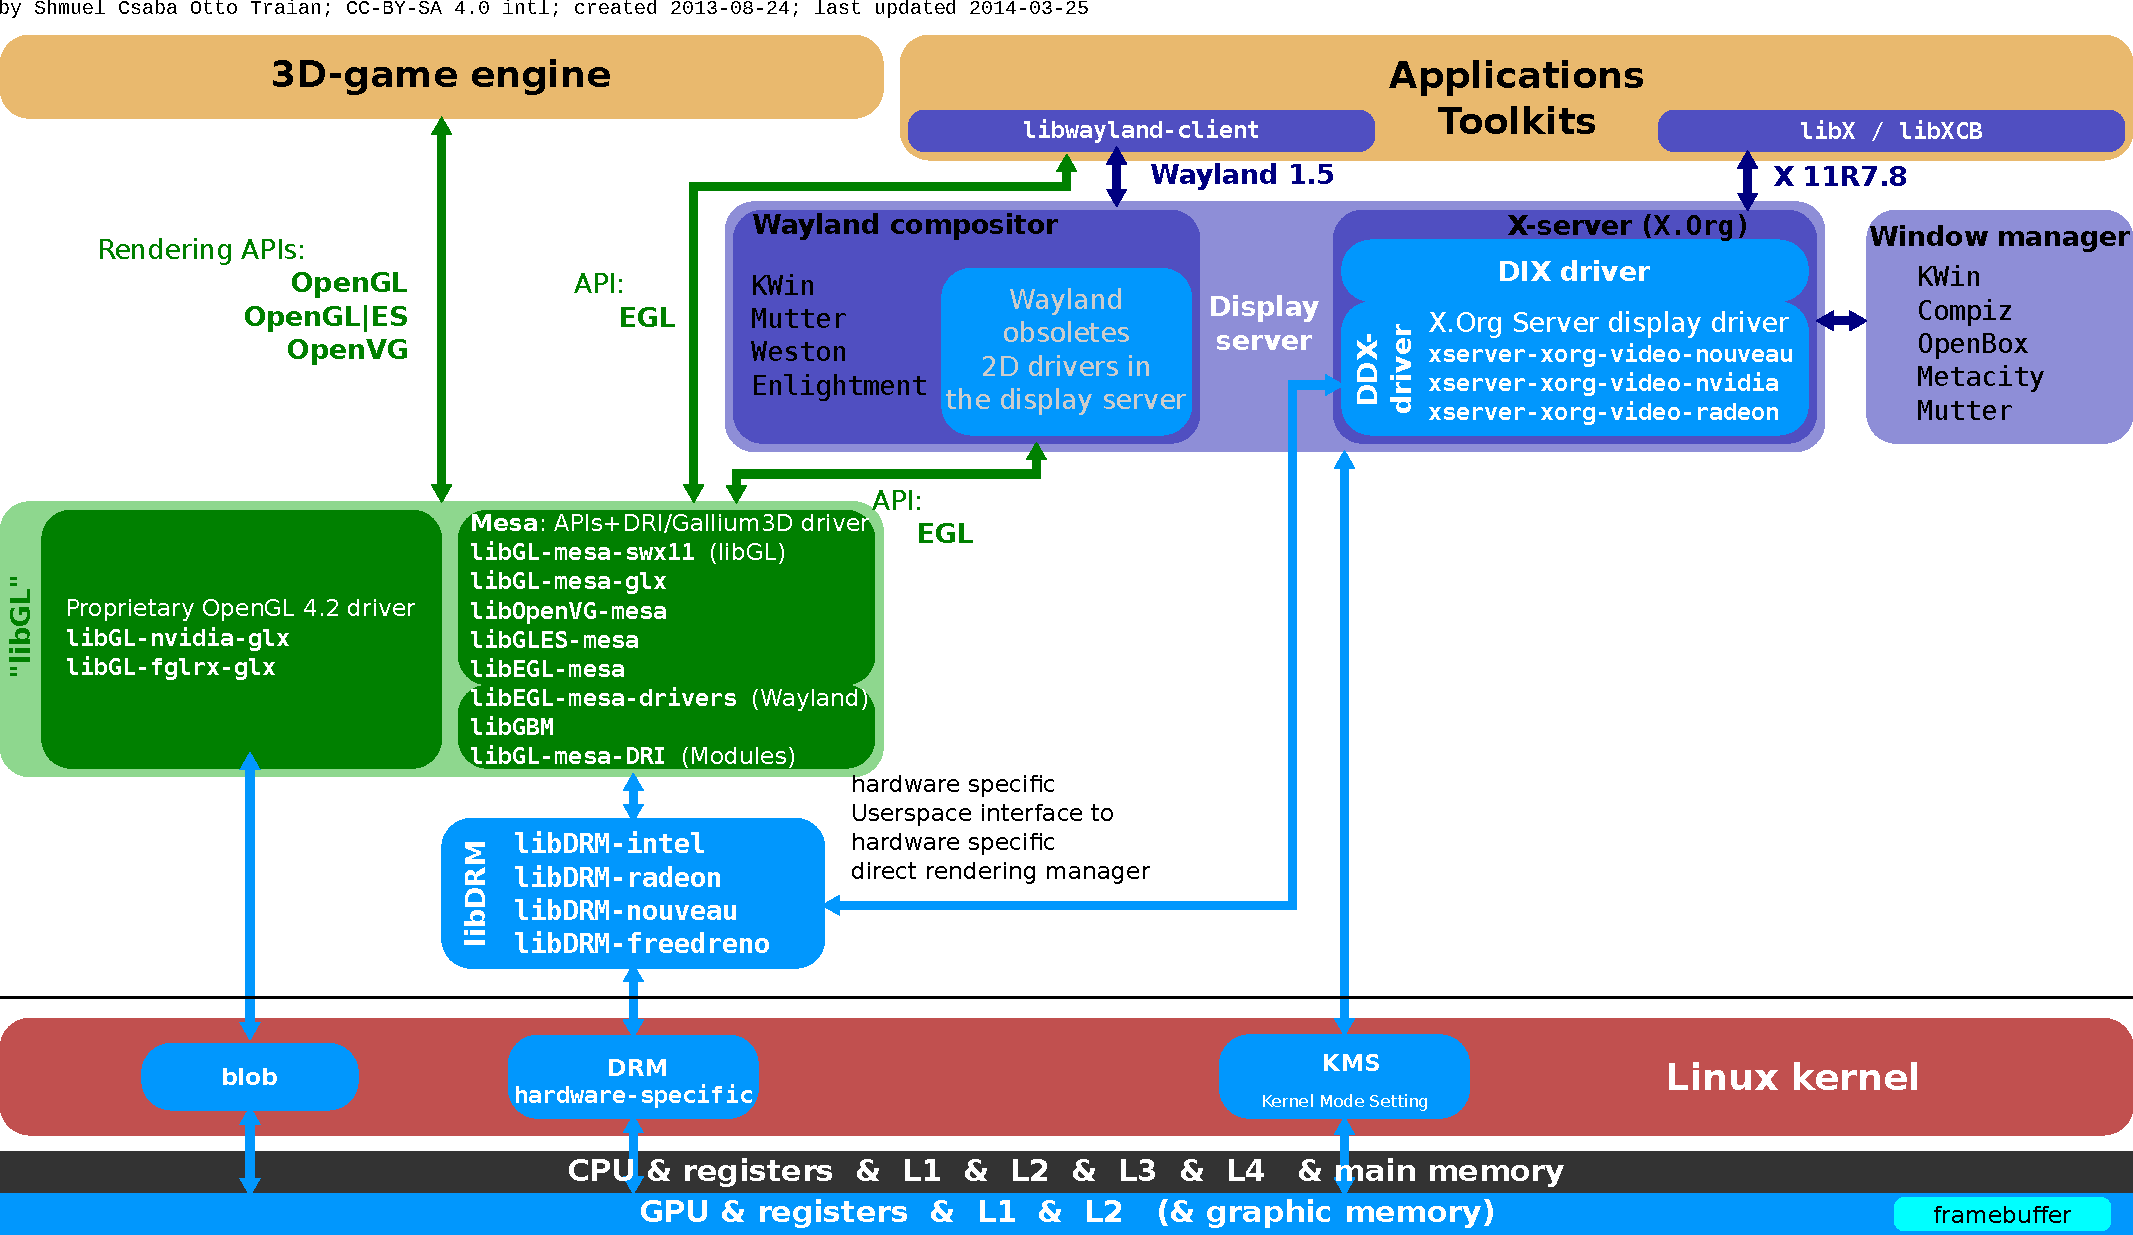
\includegraphics[width=1.02\linewidth]{imgs/Linux_Graphics_Stack_2013.pdf}
		\caption{General overview of the Linux graphics stack}
	\end{figure}
\end{frame}

\subsection{Kernel space}
\begin{frame}
	\frametitle{The kernel space}

	\begin{block}{Direct Rendering Manager (DRM) : The common code}
		\begin{itemize}
			\item This common code provides:
			\begin{itemize}
				\item Kernel ModeSetting (KMS): CRTC \& plane management;
				\item Video memory management via GEM (with a TTM backend?);
				\item Nodes with different capabilities (master or render nodes).
			\end{itemize}
		\end{itemize}
	\end{block}

	\begin{block}{DRM open source drivers}
		\begin{itemize}
			\item i810/i915: Intel;
			\item nouveau: NVIDIA;
			\item radeon: AMD/ATI;
			\item vmwgfx: VMware;
			\item many SoC GPUs (armada, exynos, msm, omap, tegra, ...).
		\end{itemize}
	\end{block}
\end{frame}

\subsection{User space}

\begin{frame}
	\frametitle{Architecture of the X-Server}

	\begin{figure}[h]
		\centering
		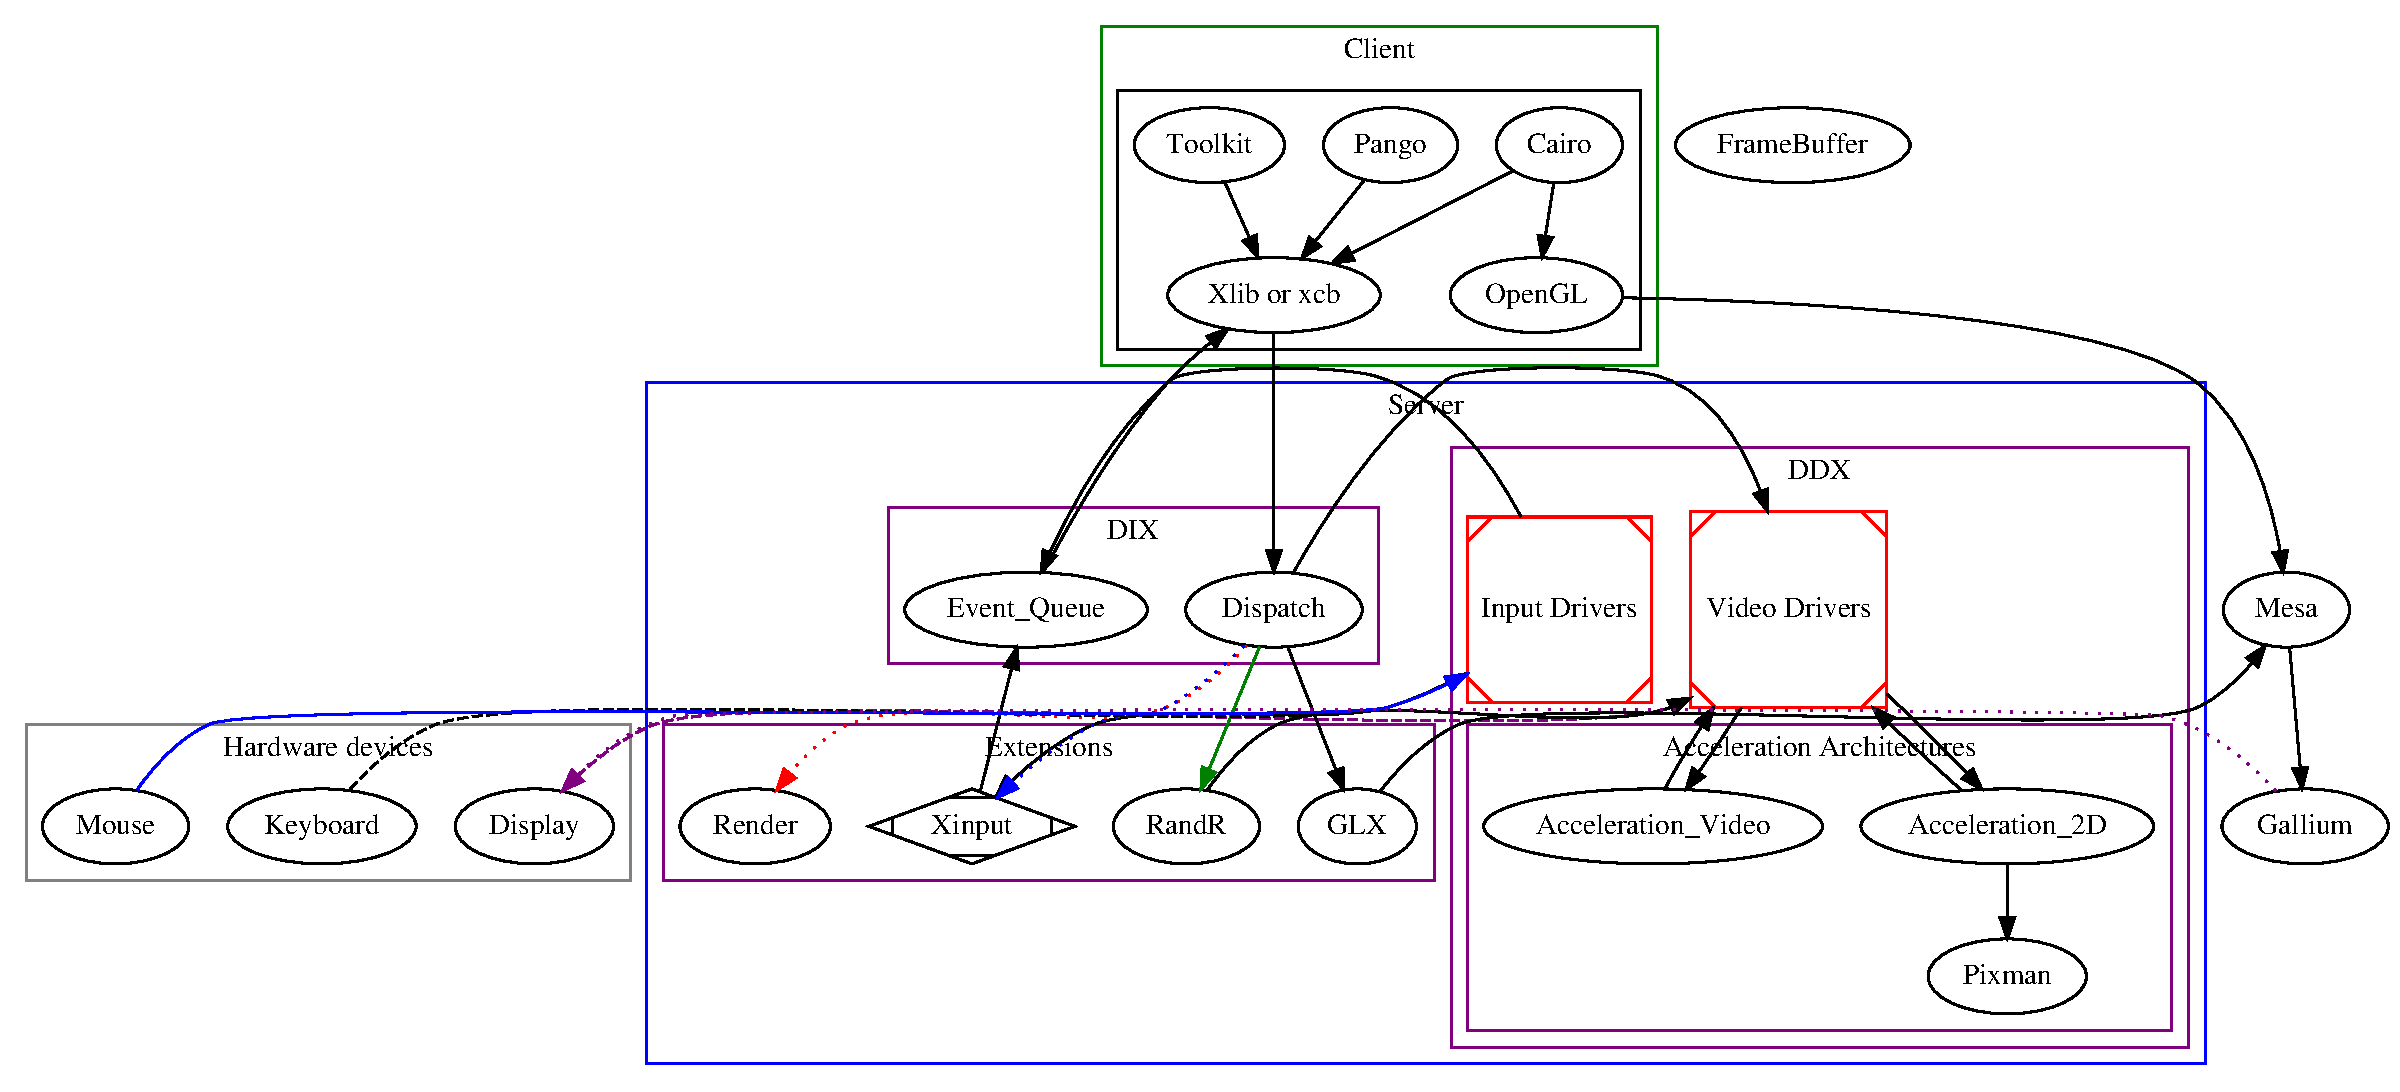
\includegraphics[width=1\linewidth]{imgs/xorg.pdf}
		\caption{General overview of the X-Server's internal architecture}
	\end{figure}
\end{frame}

\begin{frame}
	\frametitle{Architecture of Mesa}

	\begin{figure}[h]
		\centering
		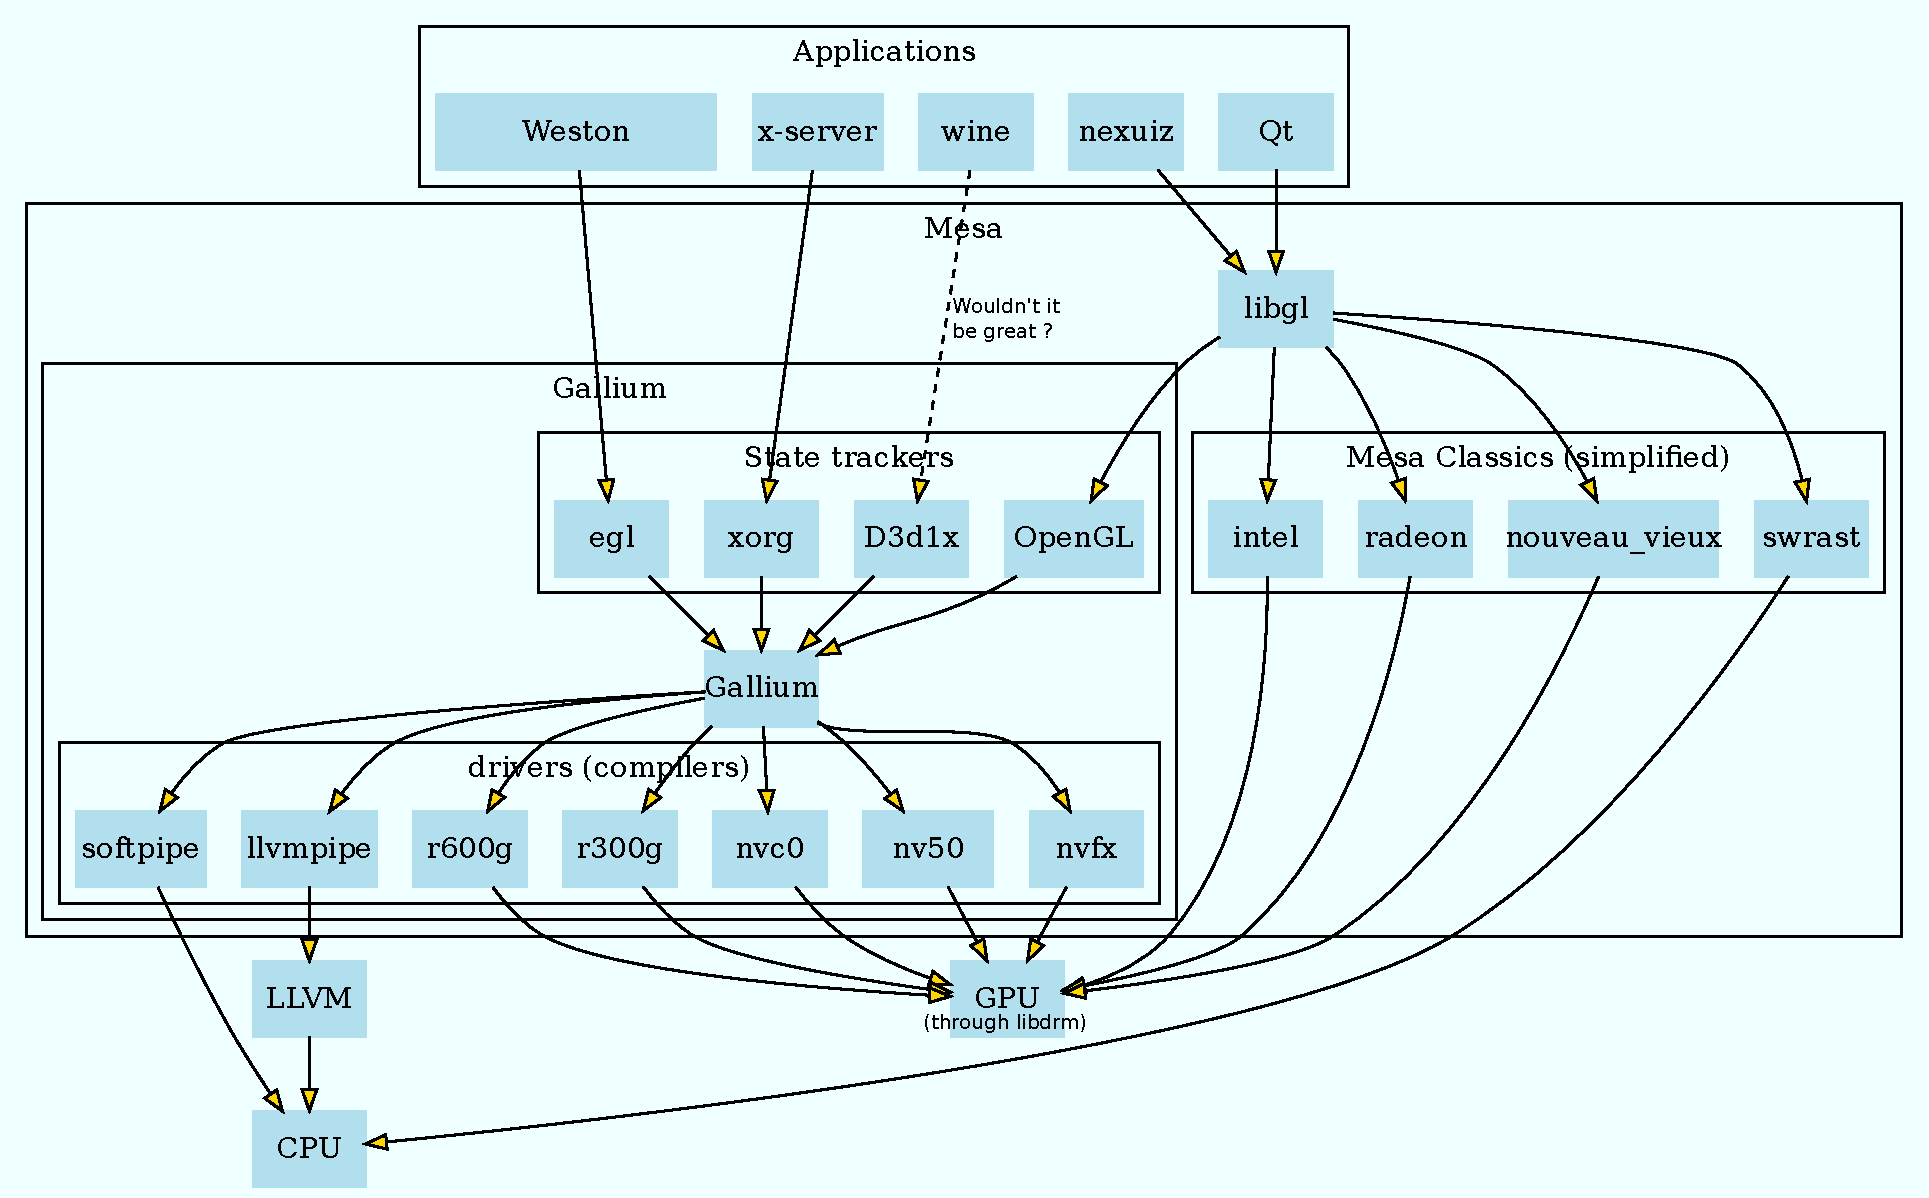
\includegraphics[width=1\linewidth]{imgs/mesa.pdf}
		\caption{General overview of Mesa's internal architecture}
	\end{figure}
\end{frame}

\section{Optimus}
\subsection{Introduction}
\begin{frame}
	\frametitle{Great performance, great battery-life}

	\begin{block}{Optimus}
		\begin{itemize}
			\item Laptops can be equipped with two GPUs;
			\item The Intel IGP is great for battery-life;
			\item NVIDIA's discrete GPU (dGPU) is great for performance;
			\item Dynamic switch between the 2: get the best of both worlds!
		\end{itemize}
	\end{block}

	\begin{block}{Challenges}
		\begin{itemize}
			\item When/How the dGPU should be turned on/off?
			\item Who drives the outputs?
			\item How to copy buffers from one driver to another?
			\item How should we do application migration?
			\item How should we handle the HDMI ``sound card''?
		\end{itemize}
	\end{block}
\end{frame}

\subsection{Turning the dGPU on/off}
\begin{frame}
	\frametitle{Turning the dGPU on/off}

	\begin{block}{How}
		\begin{itemize}
			\item Optimus laptops have ACPI functions to do that;
			\item Two ways of calling them:
			\begin{itemize}
				\item bbswitch: Old kernel module for manual management;
				\item vgaswitcheroo: Manual or automatic power management.
			\end{itemize}
		\end{itemize}
	\end{block}

	\begin{block}{When: The case of vgaswitcheroo}
		\begin{itemize}
			% \item can't remember what I wanted to write here!
			\item Turn off the dGPU when it has been idle for 5 seconds;
			\item Idle?: 
			\begin{itemize}
				\item no graphics context allocated;
				\item no output is being used;
				\item no sound interface used (not done);
				\item no call to the drm driver has been made;
			\end{itemize}
		\end{itemize}
	\end{block}
\end{frame}

\subsection{Driving the right outputs}
\begin{frame}
	\frametitle{Handling the outputs : Hardware multiplexer}

	\begin{figure}[h]
		\centering
		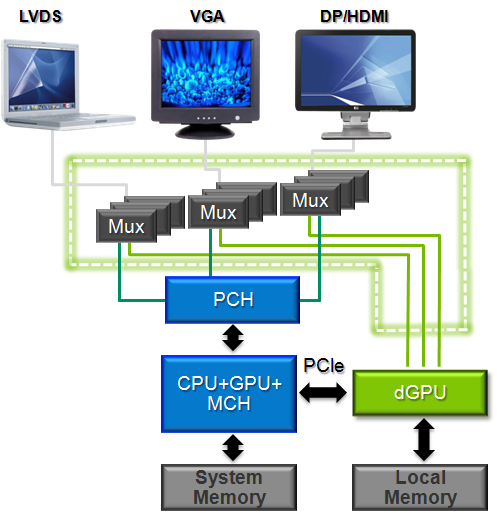
\includegraphics[height=7cm]{imgs/optimus_hw_mux.png}
		\caption{Switchable graphics}
	\end{figure}
\end{frame}

\begin{frame}
	\frametitle{Handling the outputs : Software multiplexer}

	\begin{figure}[h]
		\centering
		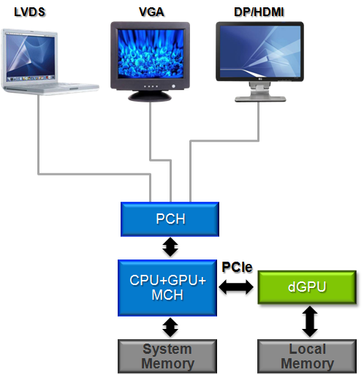
\includegraphics[height=7cm]{imgs/optimus_sw_mux.png}
		\caption{The ``real'' Optimus architecture}
	\end{figure}
\end{frame}

\subsection{How to share buffers across drivers?}

\begin{frame}
	\frametitle{Sharing buffers across drivers}

	\begin{block}{Cross-driver BO sharing : Challenges}
		\begin{itemize}
			% \item can't remember what I wanted to write here!
			\item The memory representation for buffers is different from hardware to hardware:
			\begin{itemize}
				\item pitch: number of pixels per row;
				\item tiling: technique that increases the spatial locality.
			\end{itemize}
			\item Synchronising rendering across drivers.
		\end{itemize}
	\end{block}

	\begin{block}{Solutions}
		\begin{itemize}
			\item VirtualGL: Remote rendering solution that redirects rendering commands to a distant GPU and read back to rendered frame;
			\item Primus: Same solution as VirtualGL except in a more lightweight fashion!
			\item DMA-Buf: A Linux-only solution that allows sharing buffers between different GPUs without copies.
		\end{itemize}
	\end{block}
\end{frame}

\begin{frame}
	\frametitle{Sharing buffers across drivers : VirtualGL}

	\begin{center}
		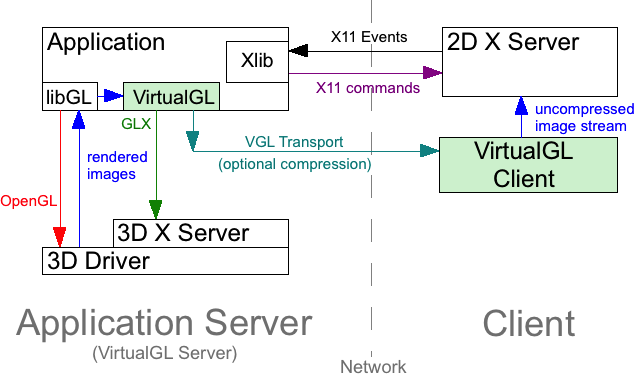
\includegraphics[width=\linewidth]{imgs/vgltransport.png}
	\end{center}
\end{frame}

\begin{frame}
	\frametitle{Sharing buffers across drivers : DMA-Buf}

	\begin{block}{Driver roles}
		\begin{itemize}
			\item Exporter: Being able to export a buffer;
			\item User: Being able to import a buffer.
		\end{itemize}
	\end{block}

	\begin{block}{General overview}
		\begin{itemize}
			\item No standardised memory allocation: It's up to the exporter;
			\item An arbitrary buffer can be wrapped into a DMA buffer;
			\item An fd can be returned to the userspace to reference this buffer;
			\item The fd can be passed to another process;
			\item The fd can be mmapped and accessed by the CPU;
			\item The fd can be imported by any driver supporting the user role.
		\end{itemize}
	\end{block}
\end{frame}

\begin{frame}
	\includegraphics[page=13,width=\linewidth]{DMA_Buffer_Sharing-_An_Introduction.pdf}
\end{frame}

\begin{frame}
	\frametitle{How should we do application migration?}

	\begin{block}{Short answer}
		\textbf{We don't!}
	\end{block}

	\begin{block}{Why?}
		\begin{itemize}
			\item The context is hardware-dependent;
			\item The context can be HUGE (hundreds of MB);
			\item The best way is to ask the application to re-upload its context: GL\_ARB\_robustness.
		\end{itemize}
	\end{block}
\end{frame}

\begin{frame}
	\frametitle{Optimus : How windows does it}

	\begin{figure}[h]
		\centering
		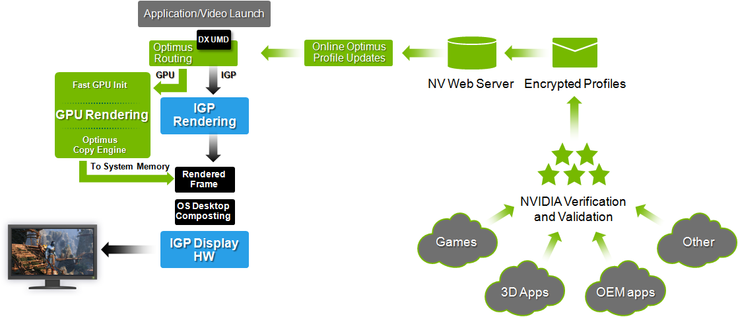
\includegraphics[width=1\linewidth]{imgs/optimus_arch.png}
		\caption{The global hardware/software infrastructure}
	\end{figure}
\end{frame}

\section{Prime}
\subsection{Introduction}
\begin{frame}
	\frametitle{Prime}

	\begin{block}{Prime}
		Prime is the name for all the ustream open source technologies
		that make hybrid graphics possible:
		\begin{itemize}
			\item DMA-Buf: sharing buffers across drivers (Linux 3.3);
			\item vgaswitcheroo: switching graphics (Linux 3.12);
			\item Cross-device fence mechanism: make a driver wait on another driver to complete a task (Linux 3.17);
			\item DMA-Buf synchronisation: Wait for rendering completion of a DMA-Buf before compositing to avoid tearing (Linux 3.19?).
		\end{itemize}
	\end{block}

	\begin{block}{List of requirements}
		\begin{itemize}
			\item running nouveau/radeon drm;
			\item running the nouveau/radeon ddx;
		\end{itemize}
	\end{block}
\end{frame}

\subsection{How to}
\begin{frame}
	\frametitle{Prime: Simplified how-to for Nouveau}

	\begin{block}{vgaswitcheroo}
		\begin{itemize}
			\item \# cd /sys/kernel/debug/vgaswitcheroo/
			\item \# cat switch
			\item \# echo (DIGD$|$DDIS) $>$ switch
			\item (Re)start your desktop environment.
		\end{itemize}
	\end{block}

	\begin{block}{XRandr}
		\begin{itemize}
			\item \$ xrandr $--$listproviders
			\item \$ xrandr $--$setprovideroffloadsink nouveau Intel
			\item This sets the order: Nouveau == offload, Intel == default
		\end{itemize}
	\end{block}
\end{frame}

\begin{frame}
	\frametitle{Prime: Simplified how-to for Nouveau}

	\begin{block}{Usage}
		\begin{itemize}
			\item DRI\_PRIME=1 glxgears \# Use the NVIDIA GPU
			\item DRI\_PRIME=0 glxgears \# Use the Intel GPU
			\item glxgears \# Use the Intel GPU
		\end{itemize}
	\end{block}

	\begin{block}{Longer How-to for Nouveau}
		\url{http://nouveau.freedesktop.org/wiki/Optimus}
	\end{block}
\end{frame}

\subsection{Demos}
\begin{frame}
	\frametitle{Prime: Demos}

	\begin{block}{Current setup}
		\begin{itemize}
			\item This is an Optimus laptop (Sandy Bridge + NVIDIA NVD9);
			\item All the outputs are connected to the Intel IGP.
		\end{itemize}
	\end{block}

	\begin{block}{List of demos}
		\begin{itemize}
			\item Selecting the GPU and checking with glxinfo;
			\item Performance difference in glxgears;
			\item Video decoding with VDPAU on the NVIDIA GPU.
		\end{itemize}
	\end{block}
\end{frame}


\section{Nouveau}
\subsection{Introduction}
\begin{frame}
	\frametitle{Nouveau: Introduction}

	\vspace{-0.3cm}
	\begin{center}
		
\includegraphics[height=3cm]{imgs/nouveau_logo.jpg}
	\end{center}
	\vspace{-0.3cm}

	\begin{block}{Nouveau: An Open Source Linux driver for NVIDIA GPUs}
		\begin{itemize}
			\item Merged in Linux 2.6.33 \& left staging on Linux 3.4;
			\item Mostly developed by Red Hat and students.
		\end{itemize}
	\end{block}

	\begin{block}{Current features}
		\begin{itemize}
			\item Modesetting support for almost all NVIDIA GPUs;
			\item 2D, 3D and video-rendering accel on NV04-;
			\item Video decoding accel on NV40-NV117 (non-free).
		\end{itemize}
	\end{block}
\end{frame}

\subsection{Current work}
\begin{frame}
	\frametitle{Nouveau: Current developments}

	\begin{block}{Current work}
		\begin{itemize}
			\item Maxwell support:
			\begin{itemize}
				\item Released in two times (March then September);
				\item Modesetting: DONE;
				\item 2D/3D support: MOSTLY DONE;
				\item Video decoding: TODO
				\item Open source firmware: WIP
			\end{itemize}
			\item Manual reclocking support:
			\begin{itemize}
				\item nv40-a3: crude support, disabled by default;
				\item nva3-ac: good chances of working;
				\item Fermi: crude support, disabled by default;
				\item Kepler: WIP, good chances of partial support;
				\item Maxwell: TODO
			\end{itemize}
			\item Adding new OpenGL extensions:
			\begin{itemize}
				\item Everything is done up to Fermi;
				\item OpenGL 4 for the other GPUs.
			\end{itemize}
		\end{itemize}
	\end{block}
\end{frame}

\subsection{Involvement from NVIDIA}
\begin{frame}
	\frametitle{Involvement from NVIDIA}

	\begin{block}{NV}
		\begin{itemize}
			\item 1998(?): NVIDIA releases ``nv'', a Linux OSS 2D driver;
			\item 1998: Obfuscation commit, release only pre-processed source.
		\end{itemize}
	\end{block}

	\begin{block}{Little hope of NVIDIA ever working again on an OSS driver}
		``It's so hard to write a graphics driver that open-sourcing it
		would not help [...] In addition, customers aren't asking for opensource drivers.''\\
		Andrew Fear, NVIDIA software product manager, April 2006
		%http://news.cnet.com/New-Linux-look-fuels-old-debate/2100-7344_3-6061491.html
	\end{block}

\end{frame}

\begin{frame}
	\frametitle{Short history of Nouveau}

	\begin{block}{Nouveau}
		\begin{itemize}
			\item 2005: Stephane Marchesin improves nv and works on 3D
			\item 2008: Open Arena runs on nv40
			\item 2009: KMS driver based on TTM for memory management
			\item 2010: Merged in Linux 2.6.33
			\item 2010: Nv is deprecated by NVIDIA, ``use VESA''.
		\end{itemize}
	\end{block}

	\begin{block}{A new hope from NVIDIA}
		\begin{itemize}
			\item September 2013: NVIDIA releases some vbios documentation;
			\item January 2014: NVIDIA starts adding support for their Tegra K1 in Nouveau, as requested by its clients;
			\item Full support for the Tegra K1 expected by the end of 2014.
		\end{itemize}
	\end{block}

\end{frame}

\section{Q\&A}
\subsection*{Q\&A}
\begin{frame}
	\frametitle{Questions?}
	\begin{block}{}
		\begin{center}
			\bigskip
			\huge Thank you for listening! Questions?
			\bigskip
		\end{center}
	\end{block}
	\vspace{20pt}
	\begin{block}{}
		\begin{center}
			\bigskip
			\large Martin Peres: martin.peres@free.fr
			\bigskip
		\end{center}
	\end{block}
\end{frame}

% DEMOS:
% - prime
% - video decoding
% - OpenGL 3.3

\end{document}
